\documentclass[tikz,border=6pt]{standalone}
\usepackage[T1]{fontenc}
\usepackage[utf8]{inputenc}
\usepackage{helvet}
\renewcommand{\familydefault}{\sfdefault}
\usetikzlibrary{arrows.meta,positioning}

\begin{document}
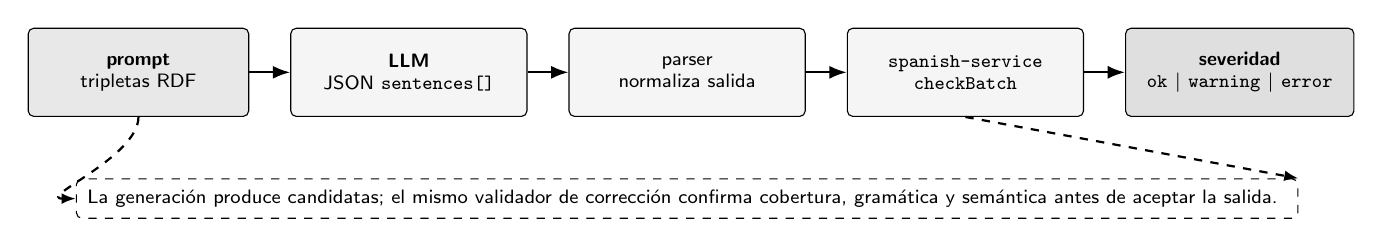
\begin{tikzpicture}[
    font=\sffamily\scriptsize,
    stage/.style={
        rectangle,
        draw=black,
        rounded corners=2pt,
        minimum width=3.0cm,
        minimum height=1.12cm,
        align=center,
        fill=gray!8
    },
    io/.style={
        rectangle,
        draw=black,
        rounded corners=2pt,
        minimum width=2.8cm,
        minimum height=1.12cm,
        align=center,
        fill=gray!18
    },
    decision/.style={
        rectangle,
        draw=black,
        rounded corners=2pt,
        minimum width=2.9cm,
        minimum height=1.12cm,
        align=center,
        fill=gray!25,
        font=\sffamily\scriptsize\bfseries
    },
    note/.style={
        rectangle,
        draw=black,
        dashed,
        rounded corners=2pt,
        align=center,
        fill=white,
        font=\sffamily\scriptsize,
        inner sep=4pt
    },
    flow/.style={-{Latex[length=2.2mm]}, thick},
    soft/.style={-{Latex[length=1.8mm]}, dashed, thick}
]

\node[io] (prompt) {\textbf{prompt}\\tripletas RDF};
\node[stage, right=0.52cm of prompt] (llm) {\textbf{LLM}\\JSON \texttt{sentences[]}};
\node[stage, right=0.52cm of llm] (parse) {parser\\normaliza salida};
\node[stage, right=0.52cm of parse] (validator) {\texttt{spanish-service}\\\texttt{checkBatch}};
\node[decision, right=0.52cm of validator] (severity) {severidad\\\texttt{ok} \textbar{} \texttt{warning} \textbar{} \texttt{error}};

\draw[flow] (prompt) -- (llm);
\draw[flow] (llm) -- (parse);
\draw[flow] (parse) -- (validator);
\draw[flow] (validator) -- (severity);

\node[note, below=0.78cm of parse, minimum width=7.8cm] (summary) {
    La generación produce candidatas; el mismo validador de corrección confirma cobertura,
    gramática y semántica antes de aceptar la salida.
};
\draw[soft] (prompt.south) to[out=-90,in=180] (summary.west);
\draw[soft] (validator.south) -- (summary.north east);

\end{tikzpicture}
\end{document}
